% ----------------------------- Design ---------------------------------------

\section{Design}

\subsection{Technical Environment}
% Mention minimum hardware configuration, software tools and package details.
\noindent
The technical environment for the project "Analyzing Social Media Posts for Mental Health Disorder Detection" comprises a combination of hardware, software, and tools that enable smooth data analysis, machine learning model training, and deployment. Below is a detailed overview of the minimum hardware configuration, software tools, and package details necessary to carry out this project effectively. \\

\noindent
\textbf{Minimum Hardware Configuration} \\
\noindent
Given the nature of the project, which involves processing textual data and training machine learning models, the hardware requirements are modest but significant enough to ensure optimal performance. The minimum configuration needed is:
\begin{itemize}
    \item \textbf{Processor} :
    \noindent
    Intel Core i5 (or equivalent) with a base clock speed of at least 2.5 GHz. A multi-core processor is preferred as it helps in parallel processing, which is essential during model training and data preprocessing steps.
    \item \textbf{RAM} :
    \noindent
    8 GB of RAM is recommended to handle the operations of data loading, cleaning, and transformation. Large datasets, like those used in this project, may require more memory to prevent memory overflow errors and reduce delays during processing. For larger datasets, 16 GB of RAM would be ideal.
    \item \textbf{Storage} :
    \noindent
    At least 256 GB of SSD storage is recommended. Faster storage access significantly impacts loading time for datasets and dependencies. SSD is preferred over traditional HDD because of its faster read/write speeds, which benefit large datasets like the Reddit-based social media posts used in this project.
    \item \textbf{Graphics Processing Unit (GPU)} :
    \noindent
    For basic machine learning tasks like Logistic Regression or SVM, a dedicated GPU is not necessary. However, if deep learning models or more complex neural networks were introduced later, a GPU like NVIDIA GTX 1060 with 4 GB VRAM or higher would be advantageous.
    \item \textbf{Operating System} :
    \noindent
    Windows 10 (64-bit) or higher, macOS 10.13 (High Sierra) or higher, or any stable Linux distribution (e.g., Ubuntu 18.04 or higher). The operating system should support all necessary machine learning libraries and be compatible with the tools required for the project.
\end{itemize} 

\noindent
\textbf{Software Tools and Packages} \\
\noindent
For the software stack, the project leverages a set of well-established tools, platforms, and programming libraries to ensure smooth execution from data preprocessing to model deployment:
\begin{itemize}
    \item \textbf{Python} :
    \noindent
    The primary programming language used for data processing, model training, and evaluation. Python is chosen due to its rich ecosystem of libraries and frameworks tailored for machine learning and data science.
    \item \textbf{Google Colab} :
    \noindent
    A cloud-based platform used for writing, executing, and sharing Python code. Google Colab provides free access to GPU and TPU resources, which is beneficial for intensive model training tasks. It also offers seamless integration with libraries like TensorFlow and PyTorch.
    \item \textbf{Jupyter Notebooks} :
    \noindent
     An alternative environment for running Python code, offering an interactive interface to write and execute code in blocks. It allows for easy visualization of results and is highly suitable for collaborative projects.
\end{itemize}

\pagebreak

\noindent
\textbf{Python Packages and Libraries}
\begin{table}[h!]
\centering
\begin{tabular}{|p{9cm}|p{6cm}|}
  \hline
  \multicolumn{1}{|c|}{\textbf{Package}} & \multicolumn{1}{c|}{\textbf{Purpose}} \\
  
  \hline
  \texttt{praw} & Access Reddit posts for data collection. \\
  
  \hline
  \texttt{pandas} & Data manipulation and analysis. \\
  
  \hline
  \texttt{textblob} & Text processing and sentiment analysis. \\
  
  \hline
  \texttt{time} & Managing execution time. \\
  
  \hline
  \texttt{re} & Regular expressions for text cleaning. \\
  
  \hline
  \texttt{TfidfVectorizer} & Convert text to TF-IDF features. \\
  
  \hline
  \texttt{stopwords} & Remove stopwords from text. \\
  
  \hline
  \texttt{tokenize} & Tokenize text data. \\
  
  \hline
  \texttt{nltk} & Natural Language Toolkit for text processing. \\
  
  \hline
  \texttt{CountVectorizer} & Convert text to Bag-of-Words features. \\
  
  \hline
  \texttt{split} & Split the dataset into training and testing sets. \\
  
  \hline
  \texttt{LogisticRegression} & Build and train Logistic Regression models. \\
  
  \hline
  \texttt{sklearn.metrics.accuracy\_score} & Calculate accuracy of the model. \\
  
  \hline
  \texttt{report} & Generate classification performance report. \\
  
  \hline
  \texttt{RandomizedSearchCV} & Hyperparameter tuning for models. \\
  
  \hline
  \texttt{seaborn} & Data visualization and plotting. \\
  
  \hline
  \texttt{matplotlib.pyplot} & Create and customize plots. \\
  
  \hline
  \texttt{matrix} & Generate confusion matrix. \\
  
  \hline
  \texttt{roc\_curve, auc, roc\_auc\_score} & Evaluate model’s ROC and AUC scores. \\
  
  \hline
  \texttt{KNeighborsClassifier} & Build k-Nearest Neighbors (k-NN) models. \\
  
  \hline
  \texttt{svm.SVC} & Build Support Vector Machines (SVM) models. \\
  
  \hline
  \texttt{naive\_bayes.MultinomialNB} & Build Naive Bayes models. \\
  
  \hline
  \texttt{scipy.stats.uniform} & Statistical operations for tuning models. \\
  
  \hline
  \texttt{RandomForestClassifier} & Build Random Forest models. \\
  
  \hline
  \texttt{sklearn.preprocessing.label\_binarize} & Convert labels for multi-class ROC analysis. \\
  
  \hline
\end{tabular}
\end{table}



\pagebreak

\subsection{Hierarchy of Modules}
% Provide a diagram.
\begin{figure}[h!]  
    \centering
    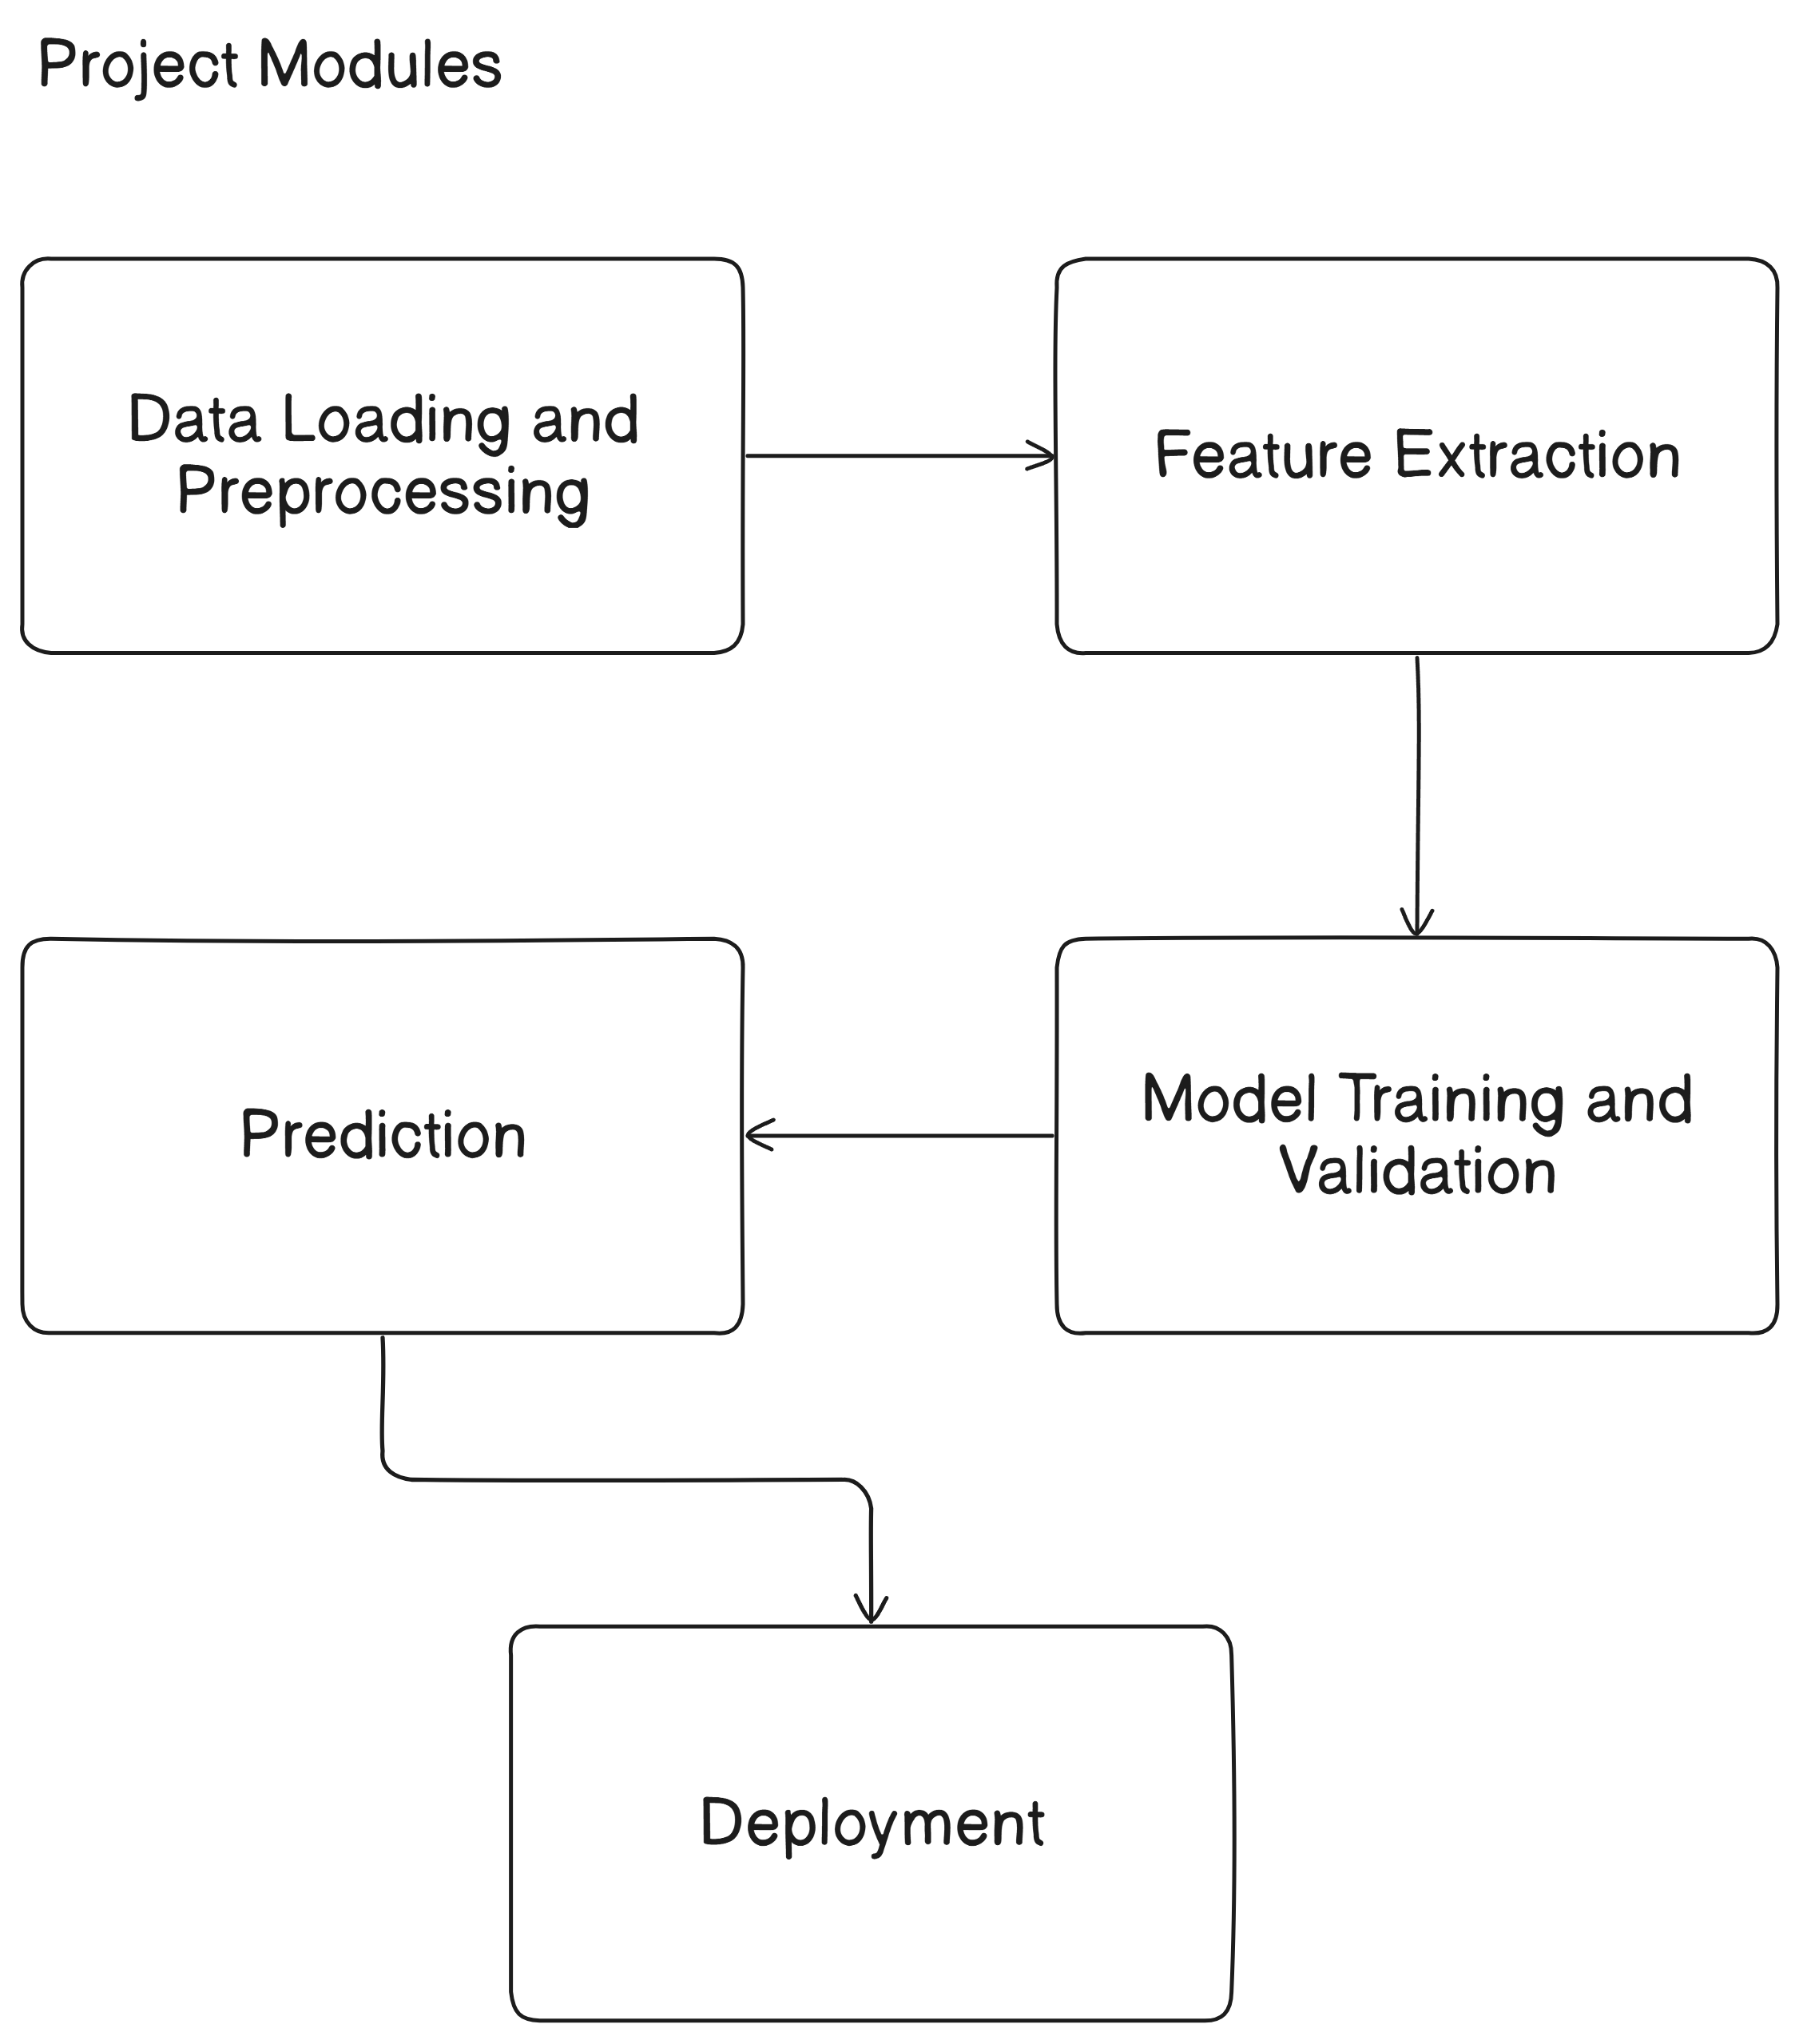
\includegraphics[width=0.6\textwidth]{Images/Project Modules.png}  
    \caption{Project Modules}
    \label{Project Modules}  % Label for referencing the figure
\end{figure}

\noindent
In this project, the system is organized into several key modules to efficiently classify mental health issues based on text input. The Data Loading and Preprocessing Module is responsible for loading the CSV data from preprocessed\_mental\_health\_text.csv and performing essential text cleaning operations, such as tokenization and stop-word removal, to prepare the data for analysis. Following this, the Feature Extraction Module employs techniques like Bag of Words or TF-IDF to convert the cleaned text into numerical features suitable for classification. The Model Training and Validation Module takes these features, splitting the dataset into training and testing sets, and implements multiple machine learning models, including Logistic Regression, k-Nearest Neighbors (k-NN), Support Vector Machines (SVM), Naive Bayes, and Random Forest. Each model is evaluated using relevant metrics to assess accuracy and performance. The Prediction Module is designed to accept new input text and utilize the trained models to predict mental health issues, ensuring that various perspectives from the different algorithms are considered. Finally, the Deployment Module offers a free solution for serving the models, potentially utilizing platforms like Google Colab or Hugging Face, allowing for real-time predictions in practical applications.

\subsection{Detailed Design}
% Provide hierarchy of modules or overall system diagram. 
% \vspace{.1in}
\begin{figure}[h!]  
    \centering
    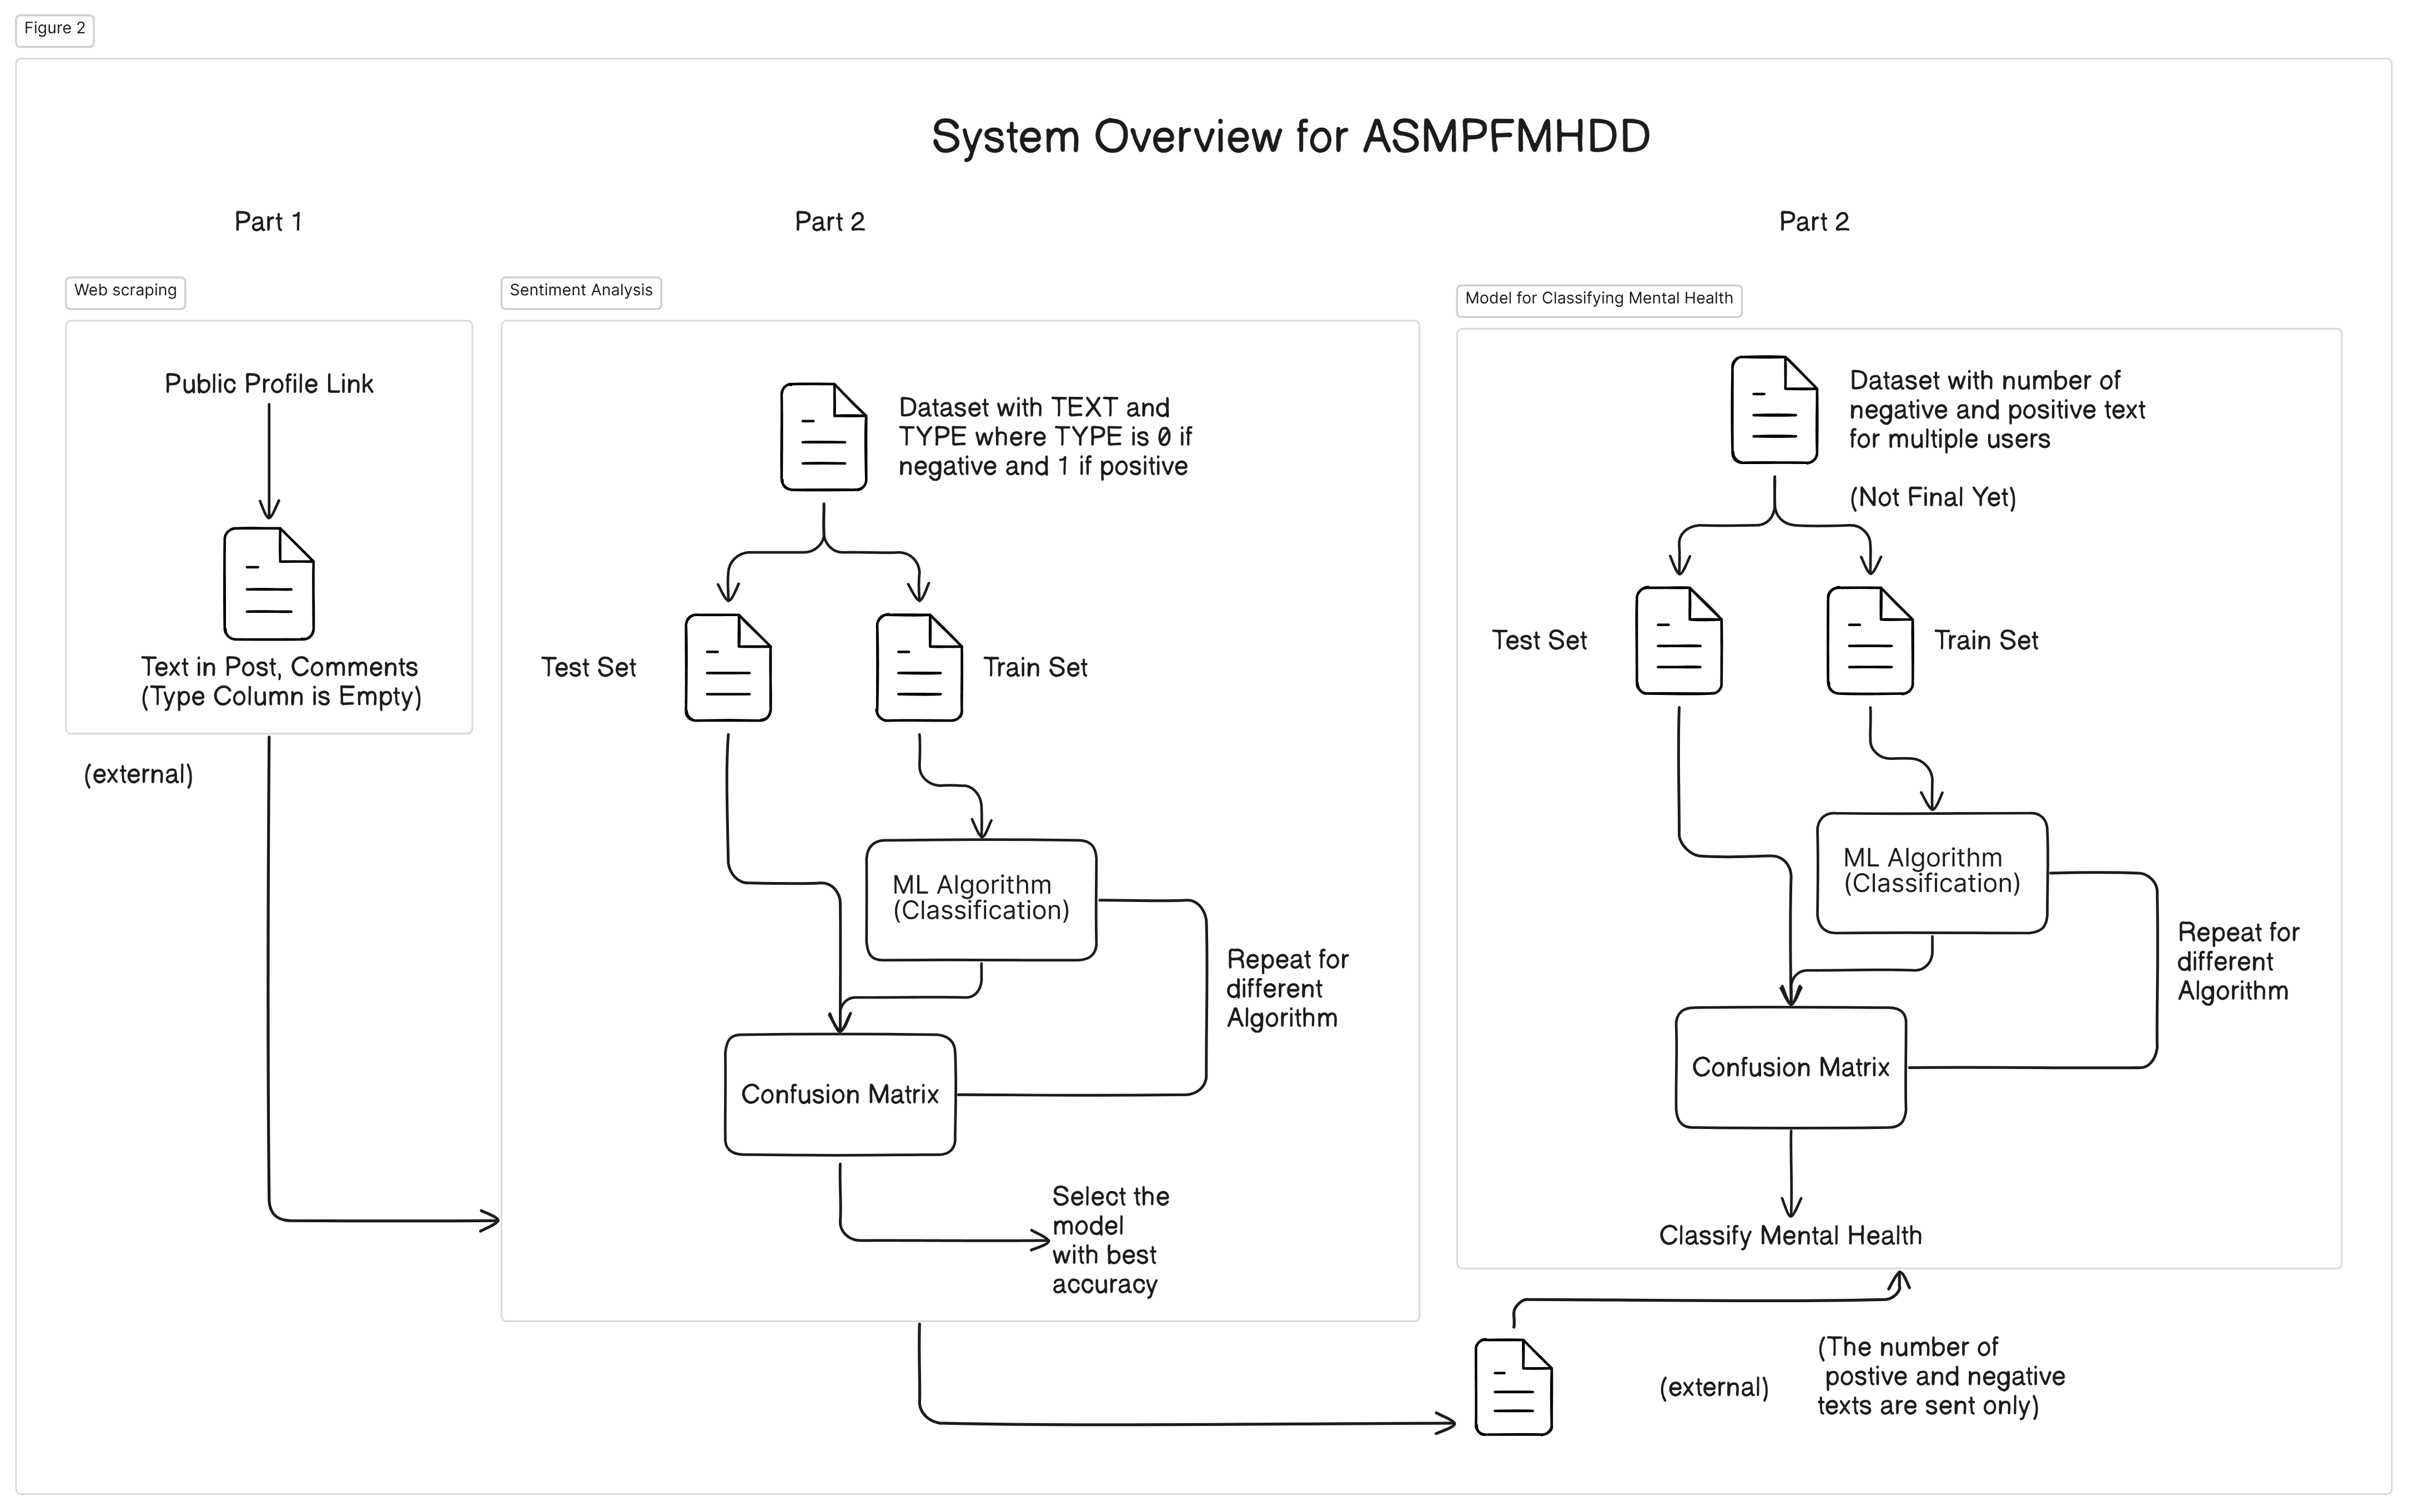
\includegraphics[width=1.0\textwidth]{Images/System Overview.png}  
    \caption{System Overview}
    \label{System Overview}  % Label for referencing the figure
\end{figure}

\begin{figure}[h!]  
    \centering
    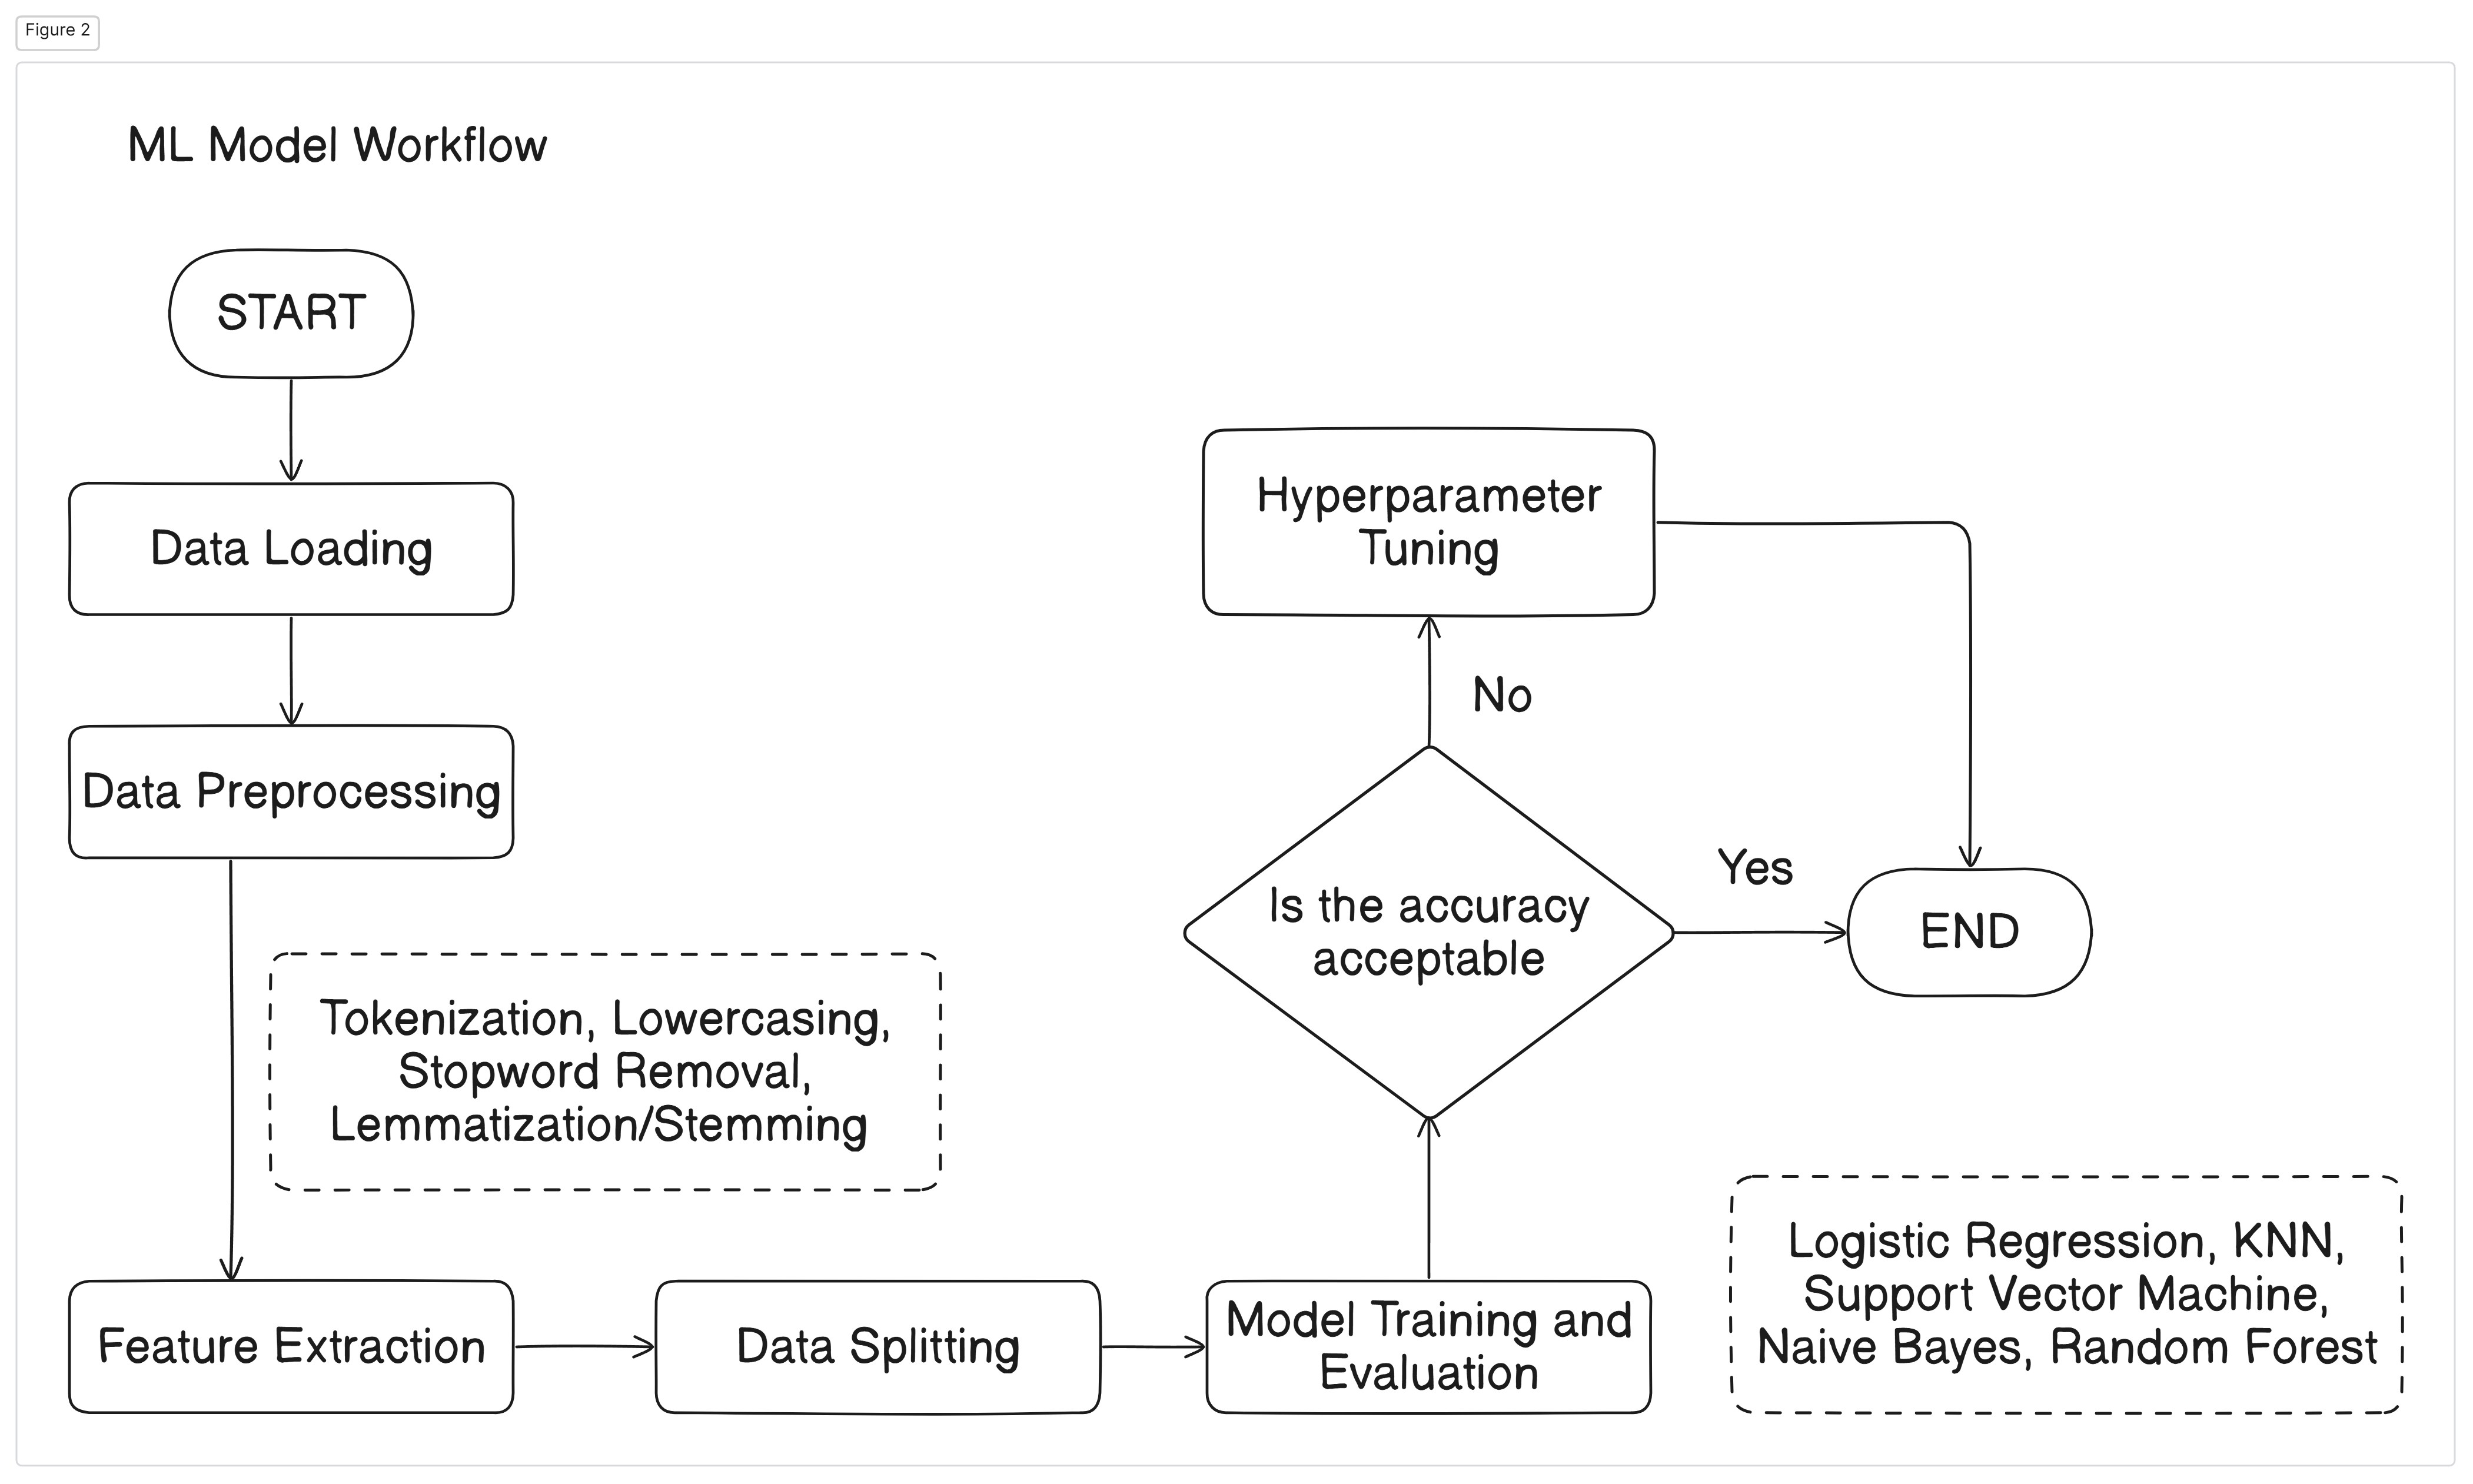
\includegraphics[width=0.95\textwidth]{Images/ML Model Workflow.png}  
    \caption{Model Workflow}
    \label{Model Workflow}  % Label for referencing the figure
\end{figure}

% \noindent
% For Detailed Design, use flowcharts, DFD, UML or ER diagrams as applicable. Titles of s7.2.1, 7.2.2 etc. should be with the name of respective design modules. Your focus should be on: “How the requirement will be implemented in the system?” Design Reference subsection numbers should be matching as stated in Requirement Matrix.
\vspace{.1in}

\subsubsection{Data Loading and Preprocessing}
\noindent
The Data Loading and Preprocessing Module is the foundation of the system, responsible for ingesting and preparing the text data for analysis. This module begins by loading the dataset from the preprocessed\_mental\_health\_text.csv file, which contains various mental health-related text entries. Once the data is loaded, a series of preprocessing steps are conducted to ensure the text is clean and ready for feature extraction. This includes tokenization, where the text is split into individual words or tokens, and lowercasing to maintain uniformity across the dataset. Additionally, stop-word removal is performed to eliminate common words that do not contribute to the meaning, such as "and," "the," and "is." Finally, lemmatization or stemming is applied to reduce words to their base or root forms. These preprocessing techniques are crucial as they help improve the quality of the input data, ultimately leading to better model performance.

\subsubsection{Feature Extraction}
\noindent
In the Feature Extraction Module, the preprocessed text data is transformed into a numerical format that machine learning algorithms can process. This module allows for the selection between two primary feature extraction methods: Bag of Words (BoW) and Term Frequency-Inverse Document Frequency (TF-IDF). The Bag of Words model creates a representation of the text based on the frequency of words, disregarding the order in which they appear, which simplifies the input for classification algorithms. Alternatively, the TF-IDF approach evaluates the importance of words in the dataset by considering their frequency in individual documents relative to their overall occurrence across all documents. This helps in highlighting the most informative words. By converting text into numerical features, this module prepares the data for the subsequent training and validation stages, ensuring that the classification models can effectively interpret the input.

\subsubsection{Model Training and Validation}
\noindent
The Model Training and Validation Module is critical to developing a robust classification system. In this module, the dataset is split into training and testing sets to evaluate the performance of the models accurately. Various classification algorithms are employed, including Logistic Regression, k-Nearest Neighbors (k-NN), Support Vector Machines (SVM), Naive Bayes, and Random Forest. Each model is trained on the training set, which involves adjusting the model parameters based on the input features and their corresponding labels. Following training, the models undergo validation to assess their performance using various metrics such as accuracy, precision, recall, and F1-score. A decision point is included to determine if the achieved accuracy meets the project requirements. If the accuracy is deemed acceptable, the model proceeds to the deployment stage. 

\begin{figure}[h!]  
    \centering
    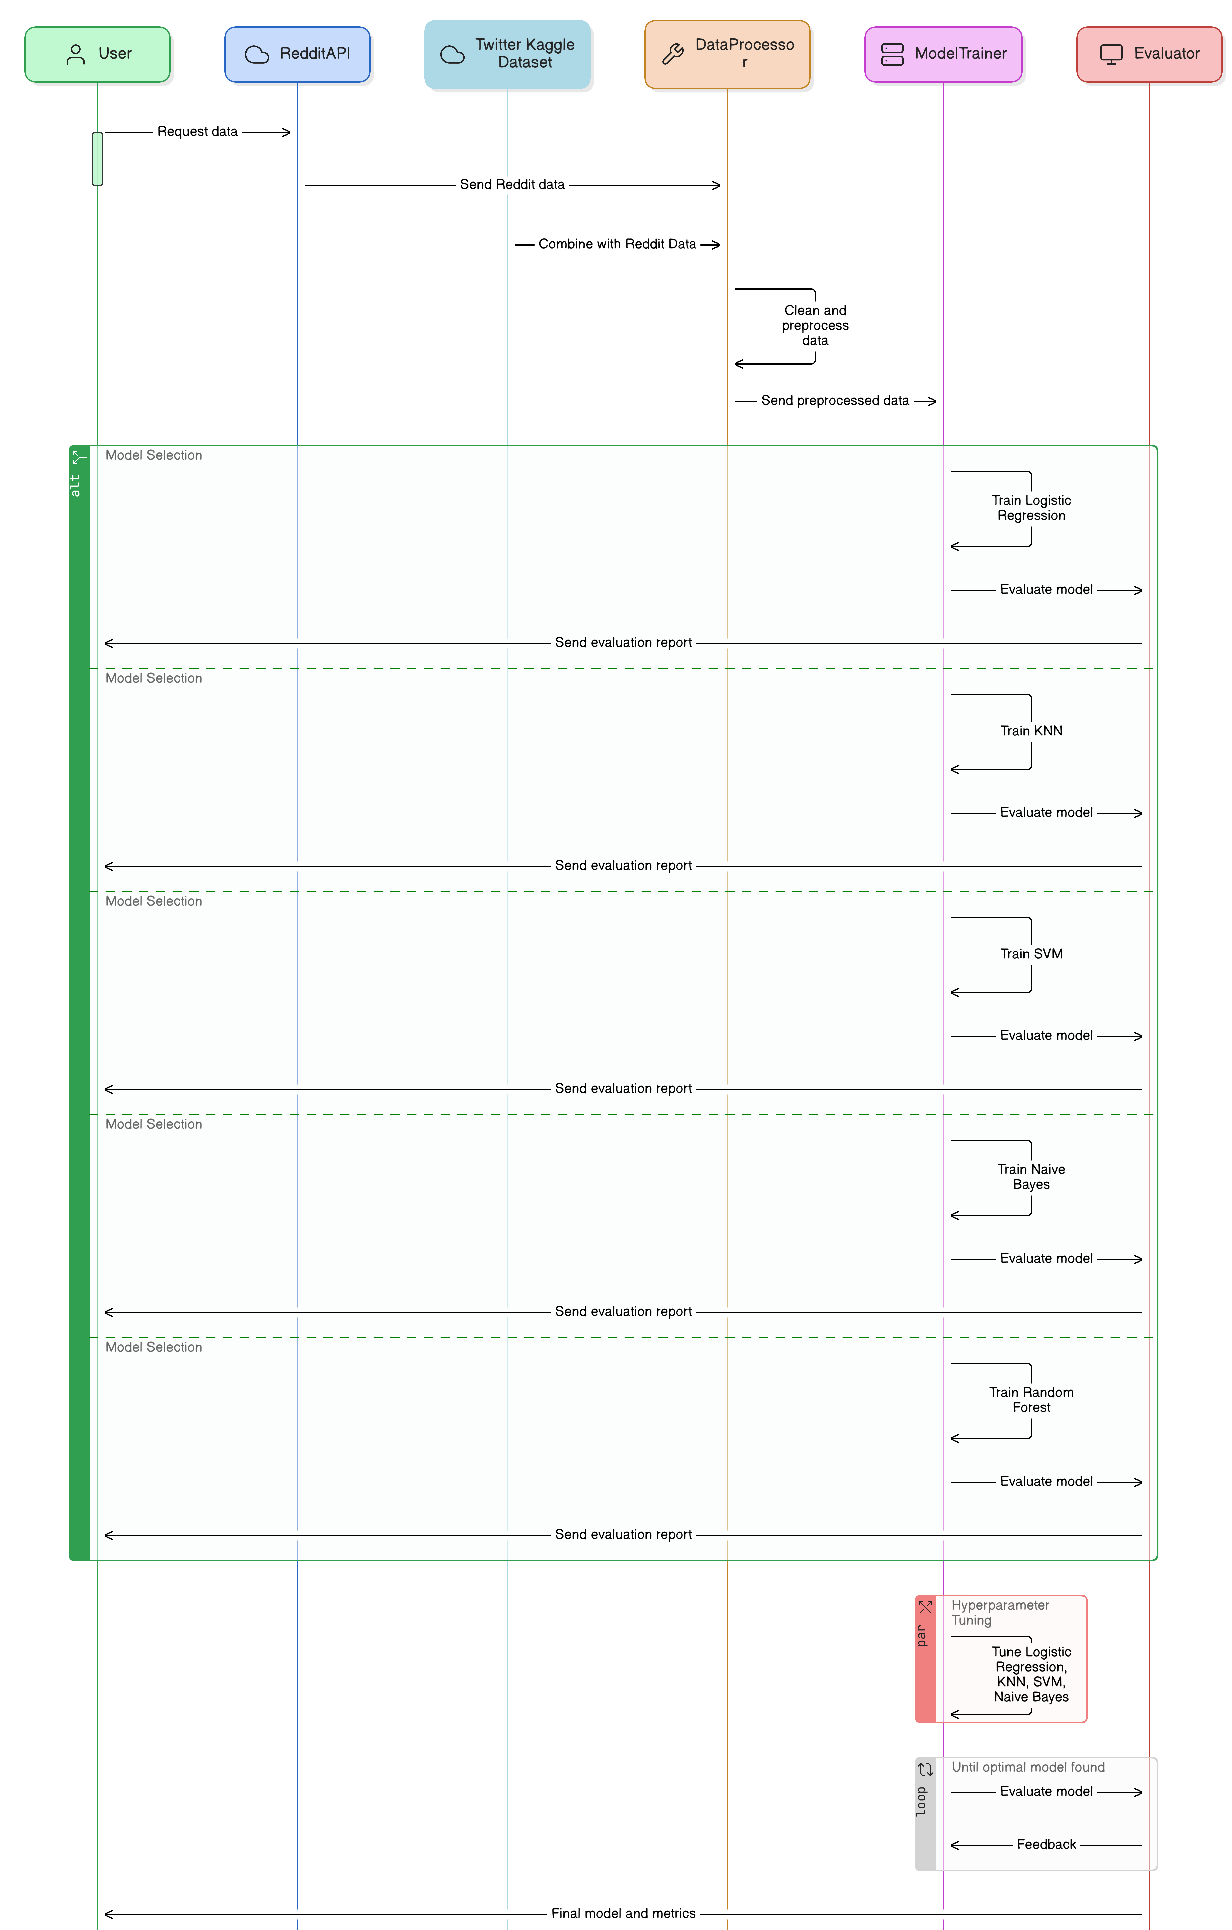
\includegraphics[width=0.85\textwidth]{Images/Project Sequence.png}  
    \caption{Project Sequence}
    \label{Project Sequence}  % Label for referencing the figure
\end{figure}

\subsubsection{Prediction}
\noindent
The Prediction Module is designed to provide real-time classification of new input text related to mental health issues. Upon receiving user input, this module initiates a preprocessing workflow that mirrors the steps applied during the training phase, including tokenization, lowercasing, stop-word removal, and lemmatization or stemming. Once the input text is preprocessed, it is fed into the trained classification models to generate predictions. Each model may provide a classification result, allowing for a comprehensive analysis of the input. This module not only delivers the predicted mental health issue but also ensures that users receive an informative output that reflects the confidence level of each prediction, enabling them to understand the model's reasoning. The seamless integration of this module into the overall system enhances the user experience by providing instant and relevant feedback.

\subsubsection{Deployment}
\noindent
The Deployment Module focuses on making the trained models accessible for real-time predictions. Once the models have been validated and selected based on their performance, this module prepares them for deployment on suitable platforms, such as Google Colab or Hugging Face. This involves packaging the models and creating a user interface where users can input text and receive predictions. The deployment process also includes considerations for scaling, ensuring that the system can handle multiple requests simultaneously while maintaining responsiveness. By providing a free and efficient deployment solution, this module enables users to access the mental health classification service easily. The deployment of the models ensures that the insights generated from the analysis can be utilized effectively in real-world applications, contributing to better mental health awareness and support.

% \noindent
% Create separate sections for separate modules of design as in Requirement Matrix. Ensure to provide Design Diagrams \textit{(e.g. System overview / DFDs / ERDs etc.; cross-reference to be drawn from Chapter 6), Decision matrix (for algorithm recommendation etc.) }




% \subsubsection{Name of Design Module 1 \label{sec:design_mod1}}
% \subsubsection{Name of Design Module 2 \label{sec:design_mod2}}
% \subsubsection{Name of Design Module 3 etc \label{sec:design_mod3}}


% Refer APPENDIX A  – Prototypes \ref{sec:proto} for prototype details.


% ------------------------------ Design Ends ---------------------------------

